\section*{Report 1 — June 18, 2025}
\addcontentsline{toc}{section}{Report 1 — June 18, 2025}

{\Huge\bfseries \hspace{2em}Setup\par}
\phantomsection
\addcontentsline{toc}{subsection}{Setup}
\vspace{0.5em}

For \( N \) assets indexed by \( i \in \{1, \dots, N\} \) observed over \( T+1 \) days indexed by \( t \in \{0, \dots, T\} \), let \( p_i^t \) denote the closing price of asset \( i \) on day \( t \).

We define the return ratio of asset \( i \) at day \( t \) as:
\begin{equation}
    r_i^t = \frac{p_i^t - p_i^{t-1}}{p_i^{t-1}} \quad \text{for } t = 1, \dots, T
\end{equation}

The average return vector \( \mu \in \mathbb{R}^N \) is given by:
\begin{equation}
    \mu_i = \mathbb{E}[r_i] = \frac{1}{T} \sum_{t=1}^T r_i^t
\end{equation}

The covariance matrix \( \Sigma = [\sigma_{ij}] \in \mathbb{R}^{N \times N} \) is defined as:
\begin{equation}
    \sigma_{ij} = \mathbb{E}[(r_i - \mu_i)(r_j - \mu_j)] = \frac{1}{T-1} \sum_{t=1}^T (r_i^t - \mu_i)(r_j^t - \mu_j)
\end{equation}

Let the current price of asset \( i \) be \( P_i = p_i^T \), and define the price vector at time \( T \) as \( \mathbf{P} = [P_1, P_2, \dots, P_N]^T \).

Suppose we are given a total budget \( B \in \mathbb{R} \).

{\Huge\bfseries \hspace{2em}Problem\par}
\phantomsection
\addcontentsline{toc}{subsection}{Problem}
\vspace{0.5em}

We seek a portfolio allocation vector \( \mathbf{x} \in \mathbb{R}^N \) that maximizes the trade-off between expected return and risk.

The optimization problem is:
\begin{equation}
    \begin{aligned}
    \max_{\mathbf{x}} \quad & ( \mu^T \mathbf{x} - q \cdot \mathbf{x}^T \Sigma \mathbf{x} ) \\
    \text{s.t.} \quad & \mathbf{P}^T \mathbf{x} = B
    \end{aligned}
    \label{eq:opt_problem}
\end{equation}

Here, \( q \in \mathbb{R} \) is a tunable hyperparameter that controls the trade-off between expected return and portfolio risk. The term \( \mu^T \mathbf{x} \) represents the expected return, while \( \mathbf{x}^T \Sigma \mathbf{x} \) corresponds to the portfolio variance.




{\Huge\bfseries \hspace{2em}Method\par}
\phantomsection
\addcontentsline{toc}{subsection}{Method}
\vspace{1.5em}

**Formulation based on \href{https://www.nature.com/articles/s41598-023-45392-w}{this paper}.**

\subsubsection*{1. Normalize Variables for Discrete Version}
\phantomsection
\addcontentsline{toc}{subsubsection}{1. Normalize for Discrete Version}

We normalize the portfolio optimization problem for discrete encoding as follows.

Let
\begin{equation}
    P' = \frac{P}{B}, \quad \mu' = \operatorname{diag}(P') \mu, \quad \Sigma' = \operatorname{diag}(P') \Sigma \operatorname{diag}(P')
\end{equation}


where
\[
\operatorname{diag}([v_1, v_2, v_3, \dots]) := 
\begin{bmatrix}
v_1 & 0 & 0 & \dots \\
0 & v_2 & 0 & \dots \\
0 & 0 & v_3 & \dots \\
\vdots & \vdots & \vdots & \ddots
\end{bmatrix}
\]

For each asset \( i \), define \( d_i \) as the largest non-negative integer such that \( 2^{d_i} \leq \frac{B}{P_i} \), i.e., the maximum exponent of 2 allowed by the budget:

\begin{equation}
    d_i = \left\lfloor \log_2 \left( \frac{B}{P_i} \right) \right\rfloor
\end{equation}

Let the total number of required binary variables (qubits) be:
\begin{equation}
    \text{qb} = \sum_{i=1}^N (d_i + 1)
\end{equation}

Construct the binary encoding matrix \( C \in \mathbb{R}^{N \times \text{qb}} \) as:
\begin{equation}
C = \left(
\begin{array}{cccccccccc}
2^0 & \cdots & 2^{d_1} & 0 & \cdots & 0 & \cdots & 0 & \cdots & 0 \\
0 & \cdots & 0 & 2^0 & \cdots & 2^{d_2} & \cdots & 0 & \cdots & 0 \\
\vdots & \ddots & \vdots & \vdots & \ddots & \vdots & \ddots & \vdots & \ddots & \vdots \\
0 & \cdots & 0 & 0 & \cdots & 0 & \cdots & 2^{0} & \cdots & 2^{d_N}
\end{array}
\right)
\end{equation}

Then the quantized variables are:
\begin{equation}
    P'' = C^T P', \quad \mu'' = C^T \mu', \quad \Sigma'' = C^T \Sigma' C
\end{equation}

The optimization problem becomes:
\begin{equation}
    \begin{aligned}
    \max_{\mathbf{b}} \quad & \mu''^T \mathbf{b} - q \cdot \mathbf{b}^T \Sigma'' \mathbf{b} \\
    \text{s.t.} \quad & \mathbf{P}''^T \mathbf{b} = 1 \\
    & \mathbf{b} \in \{0, 1\}^{\text{qb}}
    \end{aligned}
    \label{eq:binary_opt_problem}
\end{equation}



\subsubsection*{2. Reformulate Constraint to Quadratic Programming}
\addcontentsline{toc}{subsubsection}{2. Reformulate Constraint to Quadratic Programming}

To convert the problem into unconstrained quadratic form, we add a penalty term with hyperparameter \( \lambda \in \mathbb{R} \) to enforce the budget constraint:

\begin{equation}
\max_{\mathbf{b}} \quad \mu''^T \mathbf{b} - q \cdot \mathbf{b}^T \Sigma'' \mathbf{b} - \lambda \left( \mathbf{P}''^T \mathbf{b} - 1 \right)^2
\label{eq:penalized_qp}
\end{equation}



\subsubsection*{3. Generate QUBO and Ising Form}
\addcontentsline{toc}{subsubsection}{3. Generate QUBO and Ising Form}

We rewrite the constraint as a penalty term:

\begin{align}
    (\mathbf{P}''^T \mathbf{b} - 1)^2 
    &= \left( \sum_i P''_i b_i - 1 \right)^2 \label{eq:qubo_expand1} \\
    &= \sum_i P''^2_i b_i + 2\sum_{i \ne j} P''_i P''_j b_i b_j - 2\sum_i P''_i b_i + 1 \label{eq:qubo_expand2} \\
    &= - \sum_i P''^2_i b_i + 2\sum_{i,j} P''_i P''_j b_i b_j - 2\sum_i P''_i b_i + 1 \label{eq:qubo_expand3}
\end{align}
    

Substituting the expansion from Equation~\eqref{eq:qubo_expand3} into the objective in Equation~\eqref{eq:penalized_qp}, we obtain:

\begin{equation}
\max_{\mathbf{b}} \quad \sum_i b_i \left( \mu''_i + \lambda(P''_i + 2P''_i) \right) 
- \sum_{i,j} b_i b_j \left( q \cdot \Sigma''_{ij} + 2\lambda P''_i P''_j \right)
\label{eq:qubo_objective_sum}
\end{equation}

We define the QUBO matrix \( Q \in \mathbb{R}^{\text{qb} \times \text{qb}} \) as:

\begin{equation}
Q = \operatorname{diag}(\mu'' + 2\lambda P'') + \lambda \cdot \operatorname{diag}(P'')^2 - q \cdot \Sigma'' - 2\lambda P'' P''^T
\label{eq:qubo_matrix}
\end{equation}

Then the final QUBO formulation is:

\begin{equation}
\max_{\mathbf{b} \in \{0,1\}^{\text{qb}}} \quad \mathbf{b}^T Q \mathbf{b}
\label{eq:qubo_final_form}
\end{equation}



\subsubsection*{4. Translate QUBO to Ising Hamiltonian}
\addcontentsline{toc}{subsubsection}{4. Translate QUBO to Ising Hamiltonian}

To prepare for QAOA, we convert the QUBO into an Ising Hamiltonian. Since QAOA minimizes the energy, we negate the QUBO objective:

\begin{equation}
H = -\sum_{i,j} Q_{ij} \cdot \frac{(I - Z_i)}{2} \otimes \frac{(I - Z_j)}{2}
\label{eq:ising_full}
\end{equation}

Where \( Z_i \) is the Pauli-Z operator on qubit \( i \).



\subsubsection*{5. Programming}
\addcontentsline{toc}{subsubsection}{5. Programming}

We implemented the QAOA procedure using \texttt{CUDA-Q} with the Python API, running on a local GPU setup. Both gradient-based (Adam, GradientDescent) and non-gradient-based (COBYLA) optimizers were explored.

We also investigated the choice of hyperparameters:
\begin{itemize}
    \item \( \lambda \in \mathbb{R} \): to enforce the budget constraint
    \item \( q \in \mathbb{R} \): to balance expected return and risk
\end{itemize}

For the binary encoding, each asset \( i \) uses \( d_i + 1 \) qubits to represent its discrete investment level. For example, if the first asset uses 2 qubits, its quantity is represented as the binary number \( q_1 q_0 \); if the second asset uses 3 qubits, it is encoded as \( q_5 q_4 q_3 \).

The full binary vector \( \mathbf{b} \in \{0, 1\}^{\text{qb}} \) encodes the entire portfolio as a simple concatenation \( q_0 q_1 \dots q_5 \), which is easy to implement. In future versions, this structure can be refactored for improved readability and modularity.



\newpage
{\Huge\bfseries \hspace{2em}Result\par}
\phantomsection
\addcontentsline{toc}{subsection}{Result}
\vspace{1.5em}

Both \textbf{Adam} and \textbf{COBYLA} provided favorable trade-offs:
\begin{itemize}
    \item \textbf{COBYLA} converged faster in early iterations.
    \item \textbf{Adam} achieved lower final energy and showed smoother convergence, as illustrated in Fig.~\ref{fig:optimizer_comparison}.
\end{itemize}

For larger problem sizes (10 qubits and above), we found that plain \textbf{GradientDescent}—without adaptive learning rate or momentum—performed poorly (as shown in Fig.~\ref{fig:optimizer_comparison}). This may be attributed to the highly rugged loss landscape introduced by the budget constraint, as discussed in \href{https://www.mdpi.com/1999-4893/15/6/202#:~:text=,%2C%20for%C2%A0almost%20all}{this paper} shared by Prof. Pipe.

\vspace{1em}

\begin{figure}[h]
    % \centering
    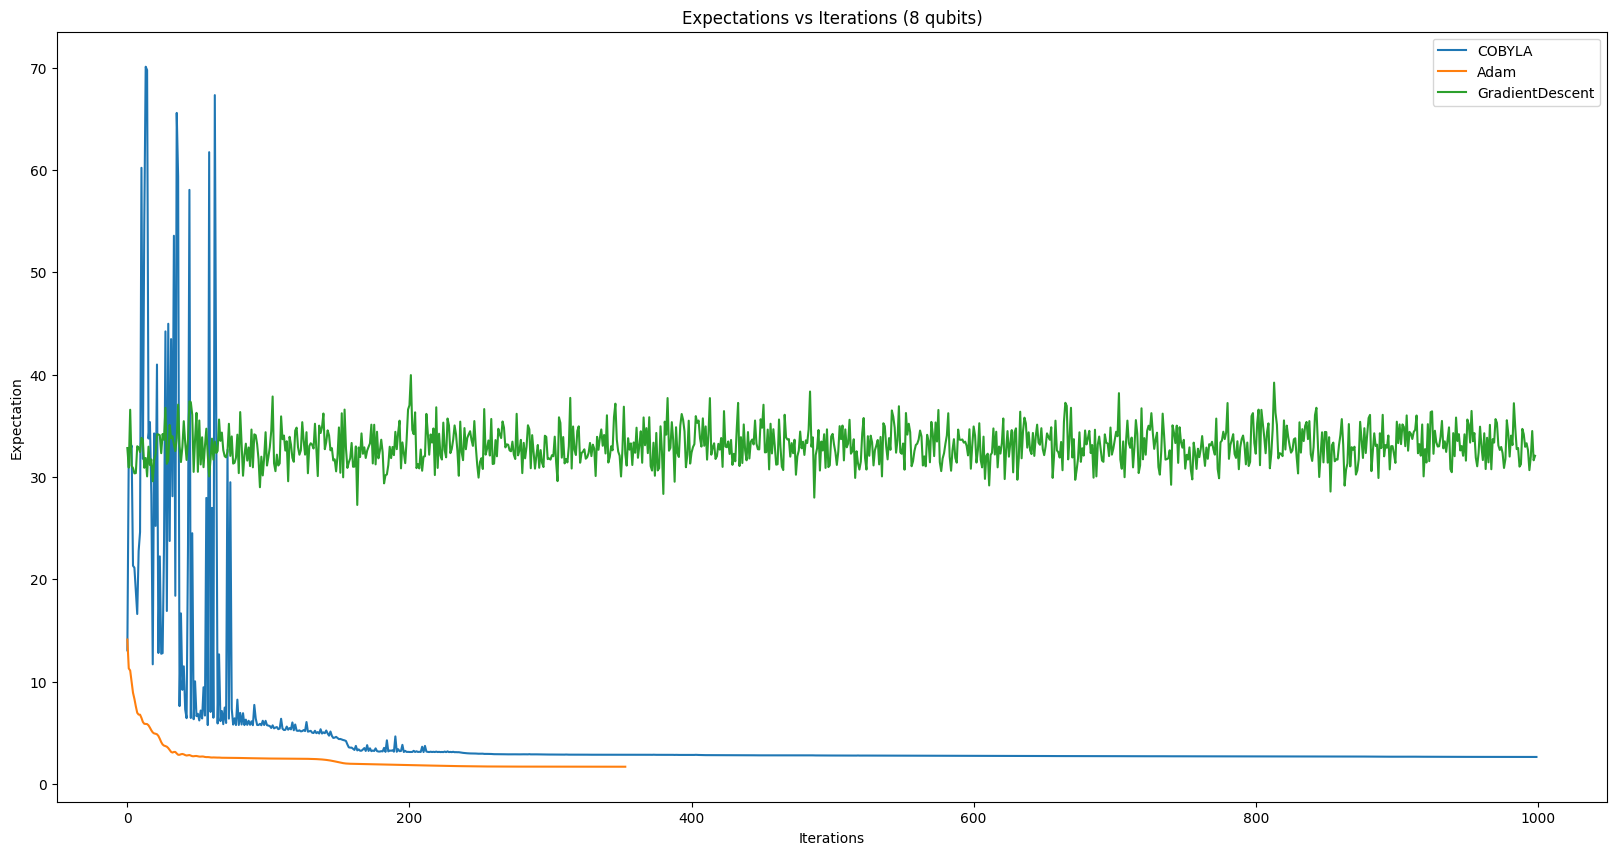
\includegraphics[width=\textwidth]{figures/report_1/optimizer_comparison.png}
    \caption{Expectation vs. Iteration for 8-qubit problem using different optimizers.}
    \label{fig:optimizer_comparison}
\end{figure}

% \vspace{1em}

Additionally, we observed that for larger budget values, it is necessary to increase \( \lambda \) to maintain a high probability of staying within the feasible region. This is because the magnitude of the return term grows with budget, requiring stronger constraint enforcement.

\vspace{1em}
\subsubsection*{Distribution Result: No Risk Case (\( q = 0 \))}
\addcontentsline{toc}{subsubsection}{Distribution Result: No Risk Case (q = 0)}

For the setup \( B = 270 \), \( P = [195, 183, 131] \), \( \mu = [0.0011, 0.0008, 0.0007] \), with \( \lambda = 3 \) and \( q = 0 \) (ignoring risk), each asset uses 1, 1, and 2 qubits respectively.

% \vspace{0.5em}
The optimal solution is to buy 2 stocks of the last asset, which gives the best return and nearly exhausts the budget. This is encoded as \( \texttt{0|0|01} = 1 \) (in base 10).

% \vspace{0.5em}
The output distribution from QAOA (executed using \texttt{CUDA-Q}) is shown in Fig.~\ref{fig:distribution_q0}.

\begin{figure}[H]
    \centering
    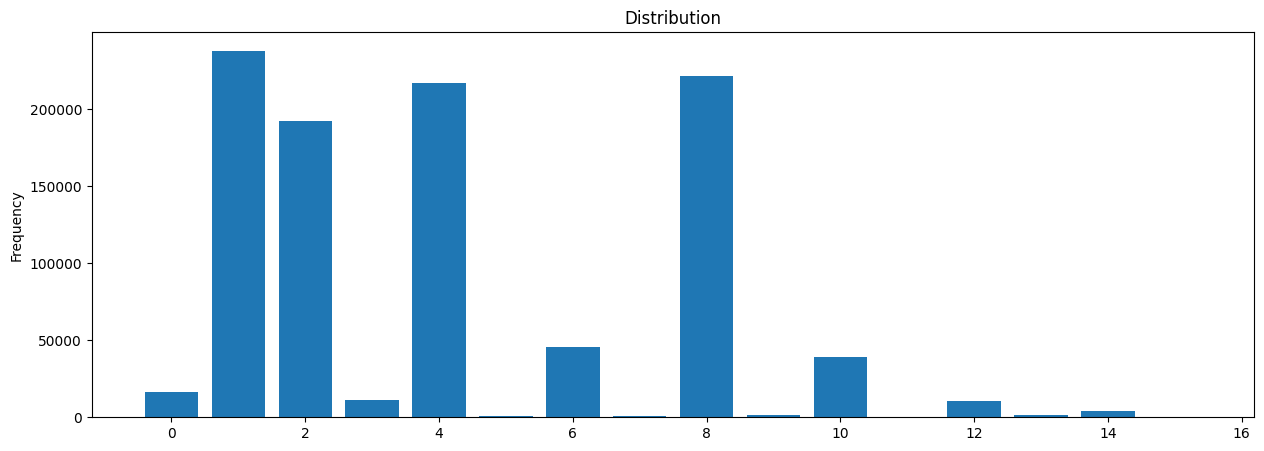
\includegraphics[width=\textwidth]{figures/report_1/distribution_q0.png}
    \caption{Distribution of measurement outcomes for QAOA with \( q = 0 \) (risk ignored).}
    \label{fig:distribution_q0}
\end{figure}

% \vspace{0.5em}
Each bar represents a binary portfolio state, interpreted as:
\begin{itemize}
    \item 0 = \texttt{0|0|00} → buy nothing
    \item 1 = \texttt{0|0|01} → buy 2 of last asset
    \item 2 = \texttt{0|0|10} → buy 1 of last asset
    \item 3 = \texttt{0|0|11} → buy 3 of last asset
    \item 4 = \texttt{0|1|00} → buy 1 of middle asset
    \item 6 = \texttt{0|1|10} → buy 1 each of middle and last
    \item 8 = \texttt{1|0|00} → buy 1 of first asset
    \item 10 = \texttt{1|0|10} → buy 1 each of first and last
    \item 12 = \texttt{1|1|00} → buy 1 each of first and middle
    \item 14 = \texttt{1|1|10} → buy 1 each of all assets
\end{itemize}